% Michał weź zrób jakieś slajdy z tymi obrazkami czy cuś
\documentclass[a4paper,12pt]{article}
\usepackage[polish]{babel}
\usepackage[utf8]{inputenc}
\usepackage[T1]{fontenc}
\usepackage{indentfirst}
\usepackage[top=2.5cm, bottom=2.5cm, left=2.5cm, right=2.5cm]{geometry}
\usepackage{amsmath}
\usepackage{hyperref}
\usepackage{graphicx}
\usepackage{listings}

\title{Symulacja ruchu drogowego na IV obwodnicy Krakowa}
\author{Szymon Gałuszka, Michał Worsowicz, Maciej Nalepa}
\date{\today}
\begin{document}
    \maketitle

    \part{Omówienie projektu}

	\section{Definicja problemu}
	
	Nasz cel to symulacja ruchu drogowego na IV obwodnicy Krakowa.
	Konieczna jest definicja tras oraz sposobu poruszania się po nich.
	Obwodnica tworzy zamkniętą pętlę (uwzględniając odcinek w budowie) i dzieli się na ruch zgodny i przeciwny do wsazówek zegara.
	
	Ruch drogowy powinien uwzględniać pojazdy osobowe, ciężarowe i transport publiczny.
	Ciężkie pojazdy obowiązują inne ograniczenia prędkości oraz zajmują więcej przestrzeni na jezdni.
	Napływ ruchu powinien odbywać się przez wjazdy na obwodnicę, które wpuszczają samochody z określoną częstotliwością, która może zależeć od pory dnia.
	
	Symulacja może obejmować wydarzenia losowe, takie jak:
	
	\begin{itemize}
		\item blokada pasa ruchu,
		\item zamknięcie zjazdu,
		\item nagłe hamowanie.
    \end{itemize}
    
    \sloppy
    \section{Obszar symulacji}
    % Obwodnica IV - szczegóły trasy
	Symulowany przez nas obszar to IV obwodnica Krakowa, znana także jako obwodnica autostradowa Krakowa, ponieważ większość jej odcinka stanowi autostrada A4.
	
	Na obwodnicy nie ma sygnalizacji świetlnej, skrzyżowania znajdują się najczęściej pod wiaduktem i najpierw należy zjechać z drogi szybkiego ruchu.
	Trasa ma zróżnicowane ograniczenia prędkości oraz różną ilość pasów ruchu.
	
	Fragment ten na zachodnich obrzeżach miasta jest dwupasmowy, a na południowych - trójpasmowy. W najbliższym czasie przewidywana jest budowa odcinka północnego, który uwzględniliśmy w naszej symulacji, odtwarzając i dodając ten fragment do projektu. Poniżej przedstawiony jest wykaz węzłów drogowych, które obejmuje symulacja (zgodnie z kierunkiem ruchu wskazówek zegara):
	
	\begin{itemize}
		\item Kraków Nowa Huta,
		\item Kraków Przewóz,
		\item Kraków Bieżanów,
		\item Kraków Wieliczka,
		\item Kraków Łagiewniki,
		\item Kraków Południe,
		\item Kraków Skawina,
		\item Kraków Tyniec,
		\item Kraków Bielany,
		\item Kraków Balice (lotnisko),
		\item Balice I,
		\item Modlniczka,
		\item Modlnica,
		\item Kraków Północ -- dla uproszczenia przyjęto taką nazwę planowanego węzła (wariant I)
	\end{itemize}

	\begin{figure}[h]
		\centering
		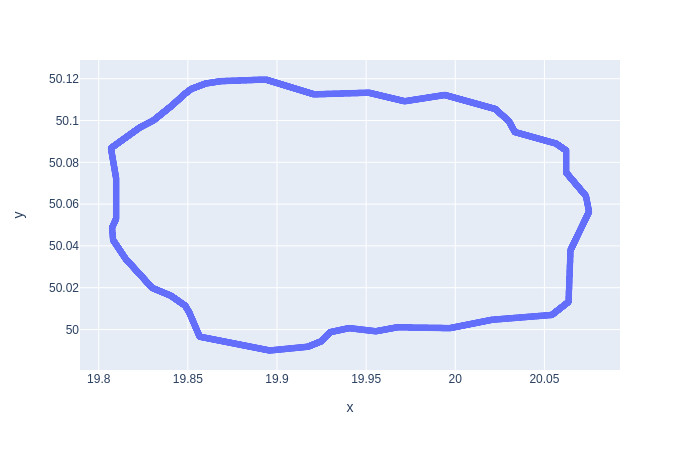
\includegraphics[width=\textwidth]{img/note-map.png}
		\caption{Mapa obwodnicy użytej w symulacji.}
	\end{figure}

    \section{Algorytm}
    % Nagel-Schreckenberg
    Zastosowany przez nas algorytm ruchu drogowego to zmodyfikowany model Nagela-Schreckenberga, będący teoretycznym modelem mikroskopowym o charakterze dyskretnym, w którym obie jednokierunkowe jezdnie są podzielone na komórki, które zawierają informację na temat ilości pasów oraz ilości pojazdów w danej chwili na jezdni. Dzięki takiemu uproszczeniu, nie jest konieczna symulacja zmiany pasu ruchu, ponieważ nie jest on określony wprost.
    
    Każda z komórek może być interpretowana na jeden ze sposobów:
    
    \begin{itemize}
    	\item komórka pusta -- fragment pustej drogi
    	\item komórka używana -- fragment zawierający pojazd na nieokreślonym pasie
    	\item komórka pełna -- fragment drogi z pojazdem na wszystkich pasach ruchu
    \end{itemize}

	Każdy samochód $n$ posiada swoją prędkość $v(n)$ o wartości liczby naturalnej, nie większej od prędkości maksymalnej $v_{max}$ -- symbolizuje ona maksymalną prędkość osiąganą przez samochód.
	
	Czas $t$ w modelu przyjmuje wartość dyskretną o stałym kroku. Nasz algorytm można podzielić na następujące po sobie czynności:

	\begin{enumerate}
		\item Losowość: \\
		Czynność ta symbolizuje wszelkie przypadki losowe z jakimi kierowca może spotkać się na drodze.
		Dla każdego samochodu $n$ prędkość może zostać zmniejszona, zwiększona lub dopasowana do ograniczenia na drodze (hamowanie lub przyspieszenie o wartość $1$ w kierunku przepisowej prędkości).
		
		\item Zwalnianie: \\
		Jeżeli odległość $d(n)$ samochodu $n$ od samochodu znajdującego się przed nim jest mniejsza od prędkości $v(n)$ tego samochodu to prędkość samochodu ulega zmniejszeniu. Jako że odległość mierzona jest w liczbie komórek, a prędkość w liczbie komórek na jednostkę czasu, to prędkość ostateczna może wynosić maksymalnie $d(n)$ na jednostkę czasu, a minimalnie zero.
		
		\item Ruch samochodu: \\
		W ostatnim kroku każdy z samochodów zostaje przesunięty do przodu o odpowiednią ilość komórek, wynikającą z jego prędkości.
	\end{enumerate}

    \part{Realizacja}
    
    \section{Struktury danych}
    % Struktura projektu
    Obsługiwany plik mapy \texttt{SimpleMap} jest w formacie \texttt{json} i przybiera następujący format:
	\begin{figure}[h]
	    \centering
	    \begin{lstlisting}
{
	"nazwa wjazdu;nazwa zjazdu": {
		"lanes": liczba_pasow,
		"maxspeed": ograniczenie_predkosci,
		"geometry": [
			[lat, lon],
			...
		]
	},
	...
}
	    \end{lstlisting}
	    \caption{Przykład pliku w formacie SimpleMap.}
	    \label{sm-format}
	\end{figure}
	Dla kompatybilności z pierwszą realizacją mapy za pomocą formatu OpenStreetMap-json powstał moduł \texttt{OpenMap}. Użycie tego formatu wymaga konwersji z formatu \texttt{.osm} do \texttt{.json}, może do tego posłużyć program JOSM.
    
    \label{automat}
    Automat komórkowy -- \texttt{Cellular} przechowuje listę następujących obiektów: pojazdów (agentów), komórek, punktów startowych i końcowych.
    Umożliwia budowanie mapy na podstawie pliku \texttt{json} kompatybilnego z modułem opracowania własnego \texttt{SimpleMap}.
    
    Komórka -- \texttt{Cell} przechowuje wskaźnik do następnej komórki, ilość dostępnych pasów, dopuszczalną prędkość oraz aktualne wykorzystanie.
    
    Logi -- \texttt{Stat} zapisuje dane w postaci ramki danych \texttt{pandas}. W każdej iteracji dopisywane są wiersze z monitorowanymi danymi.
    
    \label{logs}
    Konfiguracja -- \texttt{CONFIG} udostępniony przez moduł utils pozwala na podłączenie klasy definiującej statycznie następujące parametry:
    \begin{itemize}
    	\item Timestep -- krok czasu $t$,
    	\item Radius -- rozmiar komórki,
    	\item Spawn rate -- domyślne prawdopodobieństwo pojawienia się nowego pojazdu w danym kroku,
    	\item Agent driveoff -- prawdopodobieństwo opuszczenia obwodnicy,
    	\item Agent slow -- domyślne prawdopodobieństwo hamowania,
    	\item Agent fast -- domyślne prawdopodobieństwo przyspieszenia,
    	\item Agent limit -- domyślne prawdopodobieństwo dążenia do ograniczenia prędkości,
    	\item Agent Vmax -- domyślna maksymalna prędkość samochodu
    \end{itemize}

    \section{Implementacja}
    % Wytłumaczenie rozwiązania problemu
    
    \subsection{Mapa}
    \subsubsection{OpenStreetMap}
    Początkowo projekt zakładał wykorzystanie formatu OSM do budowania mapy. Okazało się, że dane wymagają dużego nakładu pracy w celu poprawek i wypełnienia braków (\ref{osm-na}).
    
    \begin{figure}[h]
    	\centering
    	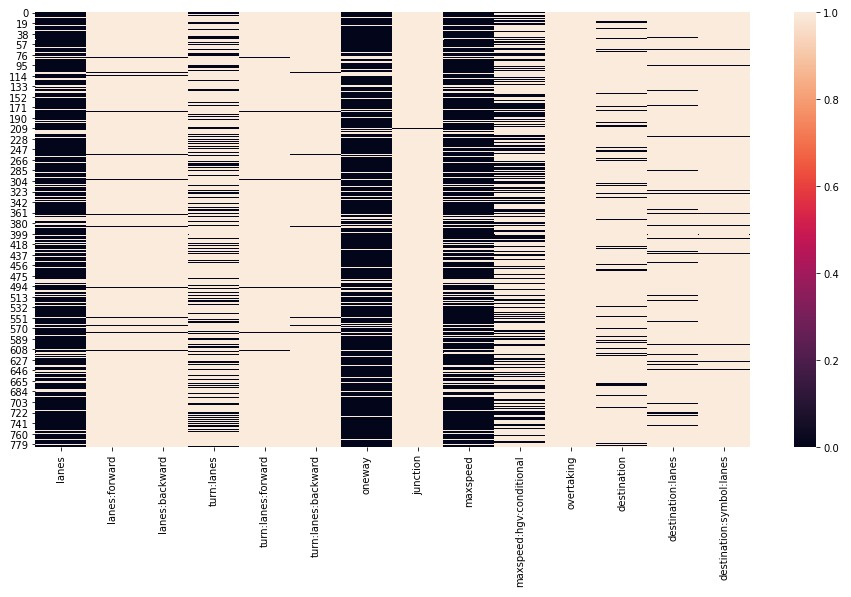
\includegraphics[width=\textwidth]{img/whiteisna.jpg}
    	\caption{Brakujące dane w pliku OSM. (biały -- oznacza brak danych | czarny -- dane występują)}
    	\label{osm-na}
    \end{figure}
    
    Ponadto, drogi OSM były podzielone na dużo bardzo krótkich odcinków (\ref{osm-parts}). Wymuszało to implementację algorytmu, który rozwiązałby istniejące relacje między odcinkami, tak aby je odpowiednio połączyć.
    
    \begin{figure}[h]
    	\centering
    	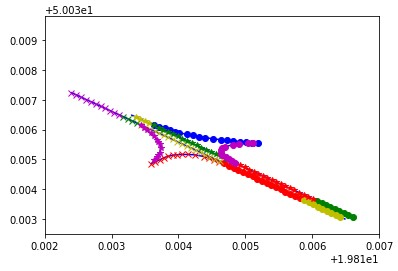
\includegraphics[width=0.7\textwidth]{img/osmparts.jpg}
    	\caption{Każdy kolor i kształt oznacza oddzielny odcinek drogi (OSM).}
    	\label{osm-parts}
    \end{figure}
    
    \subsubsection{SimpleMap}
    \texttt{SimpleMap} to moduł opracowania własnego, którego celem jest odczyt i preprocessing danych w formacie zdefiniowanym w sekcji Struktur danych (\ref{sm-format}).
    Stanowi to duże ułatwienie w pracy z mapą, ponieważ ten format jasno określa początek i koniec odcinka, co w przypadku OSM było nietrywialnym problemem.
    
    Dane dzielimy na odcinki drogi, określając sortowanie współrzędnych zgodnie lub przeciwnie do ruchu wskazówek zegara. Dodatkowe parametry to ilość pasów oraz dopuszczalna prędkość maksymalna.
    
    \begin{figure}[h]
    	\centering
    	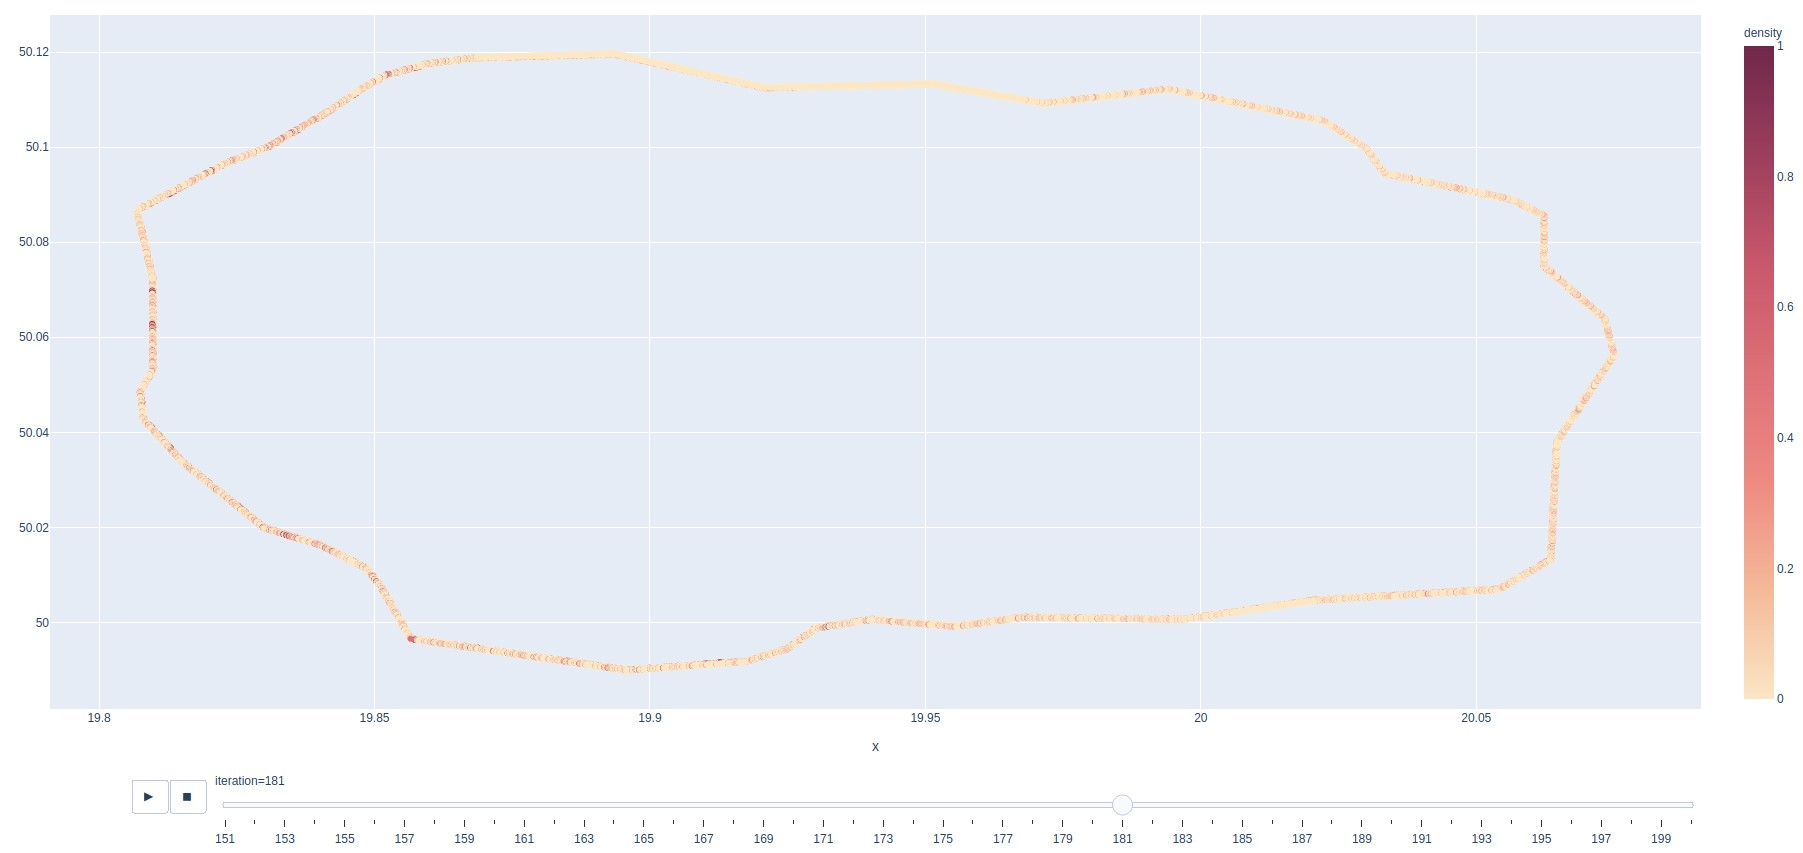
\includegraphics[width=\textwidth]{img/sim-map.jpg}
    	\caption{Animowana mapa symulacji.}
    \end{figure}
    
    \subsection{Automat komórkowy}
    Automat zdefiniowany jako \texttt{Cellular} w module \texttt{core} odpowiada za budowę mapy bazując na obiekcie \texttt{SimpleMap}. Generuje on siatkę odpowiednio połączonych komórek, tworzy przeciwny, przesunięty pas ruchu, oznacza początek i koniec drogi (od wjazdu do zjazdu) i rozwiązuje połączenia komórek między odcinkami.
    
    \begin{figure}[h]
    	\centering
    	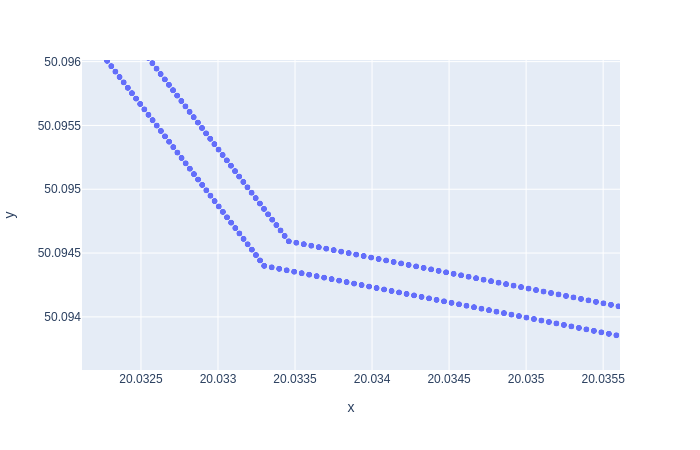
\includegraphics[width=\textwidth]{img/note-map-zoom.png}
    	\caption{Zbliżenie na komórki mapy.}
    \end{figure}

	Funkcja \texttt{step} odpowiada za obliczenie kroku symulacji. Przyjmuje ona jako parametr listę metryk (\texttt{Stat}), co umożliwia wydajne i w pełni określone przez użytkownika monitorowanie symulacji.

    \subsection{Metryki}
    W celu prowadzenia statystyk w wygodny i uniwersalny sposób opracowaliśmy klasę \texttt{Stat}.
    Aby ją wykorzystać, należy stworzyć nową klasę dziedziczącą po niej i nadpisującą definicję \texttt{extract}, która decyduje o tym jakie dane wyciągamy z aktualnego stanu symulacji i zapisujemy jako wiersze w ramce danych (\ref{logs}).
    
    Każda metryka dziedzicząca po klasie \texttt{Stat} umożliwia zapis i odczyt z pliku.
    
    Predefiniowaliśmy następujące metryki:
    \begin{itemize}
    	\item InOutFlowStat -- zapisuje ile pojazdów i gdzie opuściło lub wjechało na obwodnicę,
    	\item CellStat -- zapisuje aktualny stan wszystkich komórek mapy,
    	\item LastCellStat -- CellStat przechowujący określoną ilość iteracji wstecz,
    	\item AgentStat -- zapisuje stany wszystkich pojazdów na drodze.
    \end{itemize}
    
    \subsection{Wykresy}
    Moduł \texttt{renderer} zawiera implementację klasy \texttt{Plotter}, która umożliwia w łatwy sposób na tworzenie interaktywnych wykresów wykorzystujących bibliotekę Plotly \cite{plotly}.
    
    Dane dostarczane są w ramce danych \texttt{pandas}.
    Podstawowa klasa umożliwia tworzenie wykresów na podstawie słownika \texttt{fields}, który decyduje jakie parametry przekazujemy do Plotly Express.
    Zapewnia to dużą swobodę i jest bardzo prostym rozwiązaniem.
    
    Stworzyliśmy też trzy predefiniowane klasy do szybkiego rysowania podstawowych statystyk: AgentMetrics, FlowMetrics oraz CellularMap do rysowania aktualnej mapy.
    
    \begin{figure}[h]
    	\centering
    	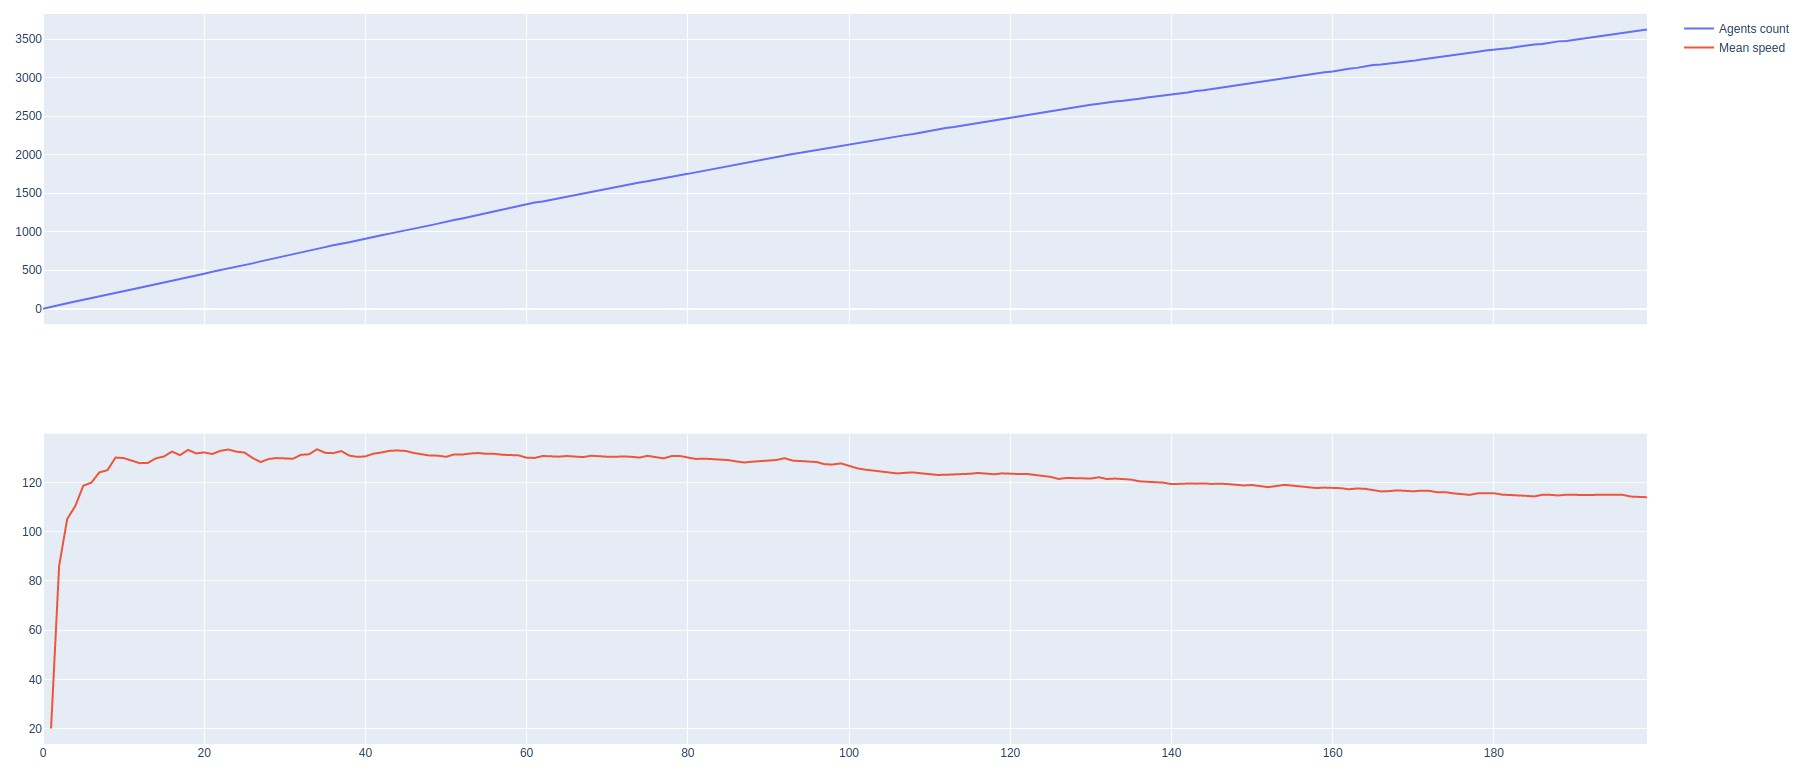
\includegraphics[width=\textwidth]{img/sim-agents.jpg}
    	\caption{AgentMetrics: Wykres na podstawie wybranych danych zebranych przez AgentStat.}
    \end{figure}
    
    \begin{figure}[h]
    	\centering
    	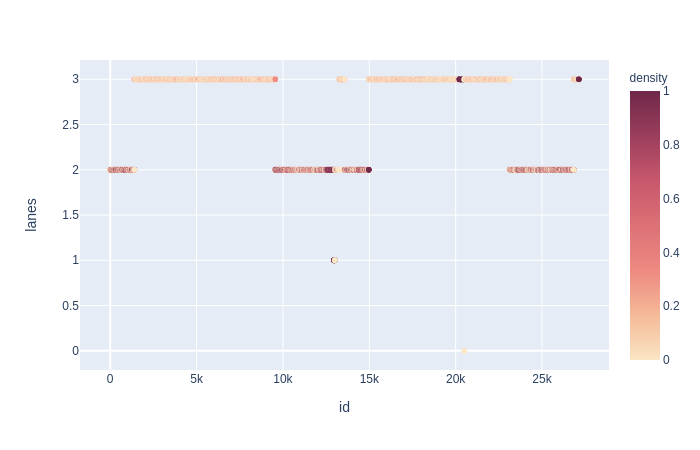
\includegraphics[width=\textwidth]{img/note-custom.png}
    	\caption{Przykładowy wykres zdefiniowany przy użyciu pola \texttt{fields}. Kod dostępny w notebooku.}
    \end{figure}

    \section{Usprawnienie}
    % Słabe punkty implementacji, co działa za wolno lub niestabilnie
    Najsłabsze punkty implementacji:
    
    \begin{itemize}
    	\item Zapis jednego stanu mapy to ramka danych o rozmiarze ilości komórek na mapie. Oznacza to, że pojedyńcza sekunda symulacji generuje nawet 30000 wpisów do ramki. W celu uniknięcia problemu z zapełnianiem pamięci stworzono specjalną klasę \texttt{LastCellStat} przechowującą określoną ilość stanów wstecz.
    	Lepszym rozwiązeniem może być zapis logów bezpośrednio do pliku.
    	
    	\item Konfiguracja prawdopodobieństwa opuszczenia skrzyżowania jest globalna, powinna być zależna od węzła.
    \end{itemize}

    \part{Podsumowanie}

    \section{Wyniki}
    % Opis symulacji i wpływu parametrów na model
    Przeprowadziliśmy symulację w trzech wariantach: normalnego ruchu, ruchu ze zwężeniem na odcinku Bielany-Balice, blokada drogi na odcinku Bieżanów-Przewóz.
    
    Symulację można powtórzyć samodzielnie za pomocą jupyter notebook \texttt{automata.ipynb} z możliwością modyfikacji parametrów.
    
    \subsection{Ruch normalny}
    \subsection{Zwężenie}
    \subsection{Blokada}
    \subsection{Statystyki}
    \subsection{Wydajność}
		
    \section{Od autorów}
    % Nasze przemyślenia o projekcie, napotkane trudności
    Nasz framework umożliwa w obecnym stanie analizę interesującego parametru: średniego czasu jaki samochód spędza na obwodnicy. Postanowiliśmy zostawić to jako propozycję do samodzielnego eksperymentu z tą symulacją.
    
    W czasie pracy napotkaliśmy duże trudności w implementacji mapy. Chcieliśmy wykorzystać istniejące, dostępne mapy, co okazało się być bardzo trudne w implementacji. Straciliśmy kilka tygodni tylko na szukanie rozwiązań umożliwiających wykorzystanie tego formatu. Ostatecznie stworzyliśmy własny, prosty format mapy, który przygotowaliśmy ręcznie na podstawie uzyskanych już wcześniej danych na temat obwodnicy.
    
    Początkowo podczas projektu stosowana była metodologia Test Driven Development (TDD), jednak tylko do czasu prac nad OpenStreetMap, z którego zrezygnowaliśmy. Ograniczenia czasowe zmusiły nas do zrezygnowania z metody, aby ograniczyć ilość pisanego kodu. Mimo to, uważamy, że wygodnie pracuje się w ten sposób i ma on potencjał do zastosowania w przyszłych projektach.

    \section{Dalsza praca}
    % Uproszczenia i części wymagające ulepszeń lub optymalizacji
    % Nie umieszczamy ich w projekcie, ale zaznaczamy od czego zacząć aby projekt usprawnić
    Aby uczynić projekt bardziej uniwersalnym, należy dodać obsługę innych zaawansowanych map.
    Można to zrobić poprzez rozbudowanie obecnego modułu \texttt{SimpleMap} lub zaimplementować obsługę znanych już formatów, np. OpenStreetMap, Google MyMaps.
    
    Projekt nie posiada innych pojazdów, niż domyślny osobowy. Zatem kolejnym usprawnieniem jest wprowadzenie pojazdów, które: 
    \begin{itemize}
    	\item obowiązują inne ograniczenia prędkości
    	\item zajmują więcej, niż jedną komórkę
    \end{itemize}

	Obsługa całej platformy może zostać zawarta w wygodnej dla użytkownika oprawie graficznej, np. \texttt{kivy}. Na chwilę obecną najbardziej interaktywny interfejs uzyskujemy poprzez \texttt{jupyter notebook}, który ma duże ograniczenia wydajności.

	\pagebreak
	\begin{thebibliography}{15}
		\bibitem{wikikrk}
		Wiki, \textit{Kraków Obwodnica IV},
		\texttt{\href{https://pl.wikipedia.org/wiki/Obwodnice_Krakowa\#IV_obwodnica}{wikipedia.org}}
		
		\bibitem{map}
		OpenStreet, \textit{mapa},
		\texttt{\href{https://www.openstreetmap.org/}{openstreetmap.org}}
		
		\bibitem{nagel}
		K. Nagel, M. Schreckenberg, \textit{Two lane traffic simulations using cellular automata},
		\texttt{\href{https://arxiv.org/pdf/cond-mat/9512119.pdf}{arxiv.org}}
		% https://www.sciencedirect.com/science/article/pii/0378437195004424
		
		\bibitem{plotly}
		Plotly, \textit{interaktywne wykresy},
		\texttt{\href{https://plotly.com/}{plotly.com}}
	\end{thebibliography}
	
\end{document}
